% TODO
% dans la section branchement multiple, dire que valeur i est de type variable
\section{Instructions de contr\^ole}
\label{sec:InstructionsDeControle}
On appelle \textit{instruction de   contr\^ole} toute instruction  qui
permet de contr\^oler la succession des actions d'un programme.  Parmi
les instructions   de  contr\^ole, on  distingue  les  instructions de
\textit{branchement} et les instructions de \textit{boucle}. L'\'etude
de ce type d'instruction va occuper cette section et la suivante.
\subsection{Les instructions de branchement conditionnel}
\label{sec:BranchementConditionnel}   
Il existe deux type d'instructions de branchement.
\subsubsection{Branchement\qquad \texttt{if \dots\ then \dots\ else}}
\label{sec:BranchementIfThenElse}
La forme g\'en\'erale d'une conditionnelle en~C est~:
\par
\begin{center}
  \begin{tabular}{l}
    \textbf{if(} \texttt{condition 1} \textbf{)}\\
    \qquad \texttt{instruction 1} \\
    \textbf{else if(} \texttt{condition 2} \textbf{)}\\
    \qquad \texttt{instruction 2} \\
    \textbf{\vdots} \\
    \textbf{else} \texttt{instruction n} \\
  \end{tabular}
\end{center}
%------------------------------------------------------------------------------
\begin{exercice}[Correction d'une erreur]
  Corriger le programme suivant~:
  \input{Verbatim/if.c.verb}
\end{exercice}
%------------------------------------------------------------------------------
\begin{exercice}[Indice de masse corporelle]
  Le statisticien et sociologue belge Qu\'etelet a observ\'e au milieu
  du~XIXi\`eme    si\`ecle,   que  le      rapport~(I)  du poids    en
  kilogrammes~(P) par la taille   en m\`etres~(T) au   carr\'e \'etait
  constant chez   des individus de   constitution moyenne.  En~$1998$,
  l'Organisation Mondiale de la Sant\'e a \'etablit une classification
  suivant ce rapport~${I=P/T^{2}}$~:
  \begin{itemize}
  \item maigreur pour~${I<18.5}$
  \item limite moyenne pour~${18.5 \ldots 24.9}$
  \item surpoids pour~${I>25}$
  \end{itemize}
  \par
  Construisez une proc\'edure qui demande  \`a l'utilisateur son poids
  en  kilogrammes  et sa  taille en m\`etres,   calcul l'indice~$I$ et
  affiche sa condition par rapport \`a la classification de l'OMS.
  \par
  N'oublions pas le seul indice qui compte~: \^etre bien dans sa peau~!
  \ifcorrection
  \begin{correction}
    \input{Verbatim/indicemassecorporelle.c.verb}
  \end{correction}
  \fi
  \paragraph{Indication~:} pour saisir au clavier un flottant et le stocker 
  dans une variable puis l'afficher, on peut s'inspirer du code~:
  \begin{verbatim}
  #include<stdio.h>
  int main(void){
     float var ;
     scanf("%f",&var) ;
     printf("%f\n",var) ;
     return 0 ;
  }
  \end{verbatim}
\end{exercice}

\begin{exercice}[Proc\'edure de tarification]
  Les tarifs d'une piscine sont les suivants~:
  \begin{itemize}
  \item trois euros si vous avez entre~$18$ et~$65$ ans~;
  \item deux euros si vous avez plus de~$65$ ans~;
  \item un euros si vous avez moins de~$18$ ans.
  \end{itemize}
  De plus, vous pouvez b\'en\'eficier  d'une r\'eduction de~$20$\%  si
  vous avez une carte de r\'eduction.
  \par\medskip\noindent
  Construire une proc\'edure principale qui  prend en entr\'ee l'\^age
  du client et un entier indiquant  s'il a une  carte (0 pour non et 1
  pour oui), et qui renvoie  la somme  \`a payer. L'exercice  consiste
  \`a compl\'eter le squelette suivant~:
\begin{verbatim}
#include <stdio.h>  /* pour afficher et saisir au clavier scanf */

int main(void){

       int    Age    ;      /* variable locale stockant l'age */
       int    Carte  ;      /* 1 si carte, 0 sinon            */
       float  APayer ;      /* variable locale stockant le r\'esultat */

       /* On collecte les donn\'ees concernant le client */
       printf("Age du client ? ") ; /* on affiche la cha\^ine a l'\'ecran */
       scanf("%d", &Age);           /* nous expliciterons plus tard la */
                                    /* syntaxe &Age                    */
       printf("Le client a-t-il une carte ? ") ;
       scanf("%d", &Carte);

       /* La partie de conditionnelle proprement dite */

       /* (a completer) */

        /* L'affichage du r\'esultat */
        printf("La somme a payer est %f",APayer) ;
        return 0 ;
}
\end{verbatim}
  Les affectations  et les op\'erations  usuelles sont classiques.  On
  affecte la  valeur~$3$  \`a la  variable  \texttt{foo}  en utilisant
  l'instructions \mbox{\texttt{foo=3.0;}} et on  a des instructions du
  type \mbox{\texttt{foo=foo*5.0;}}.
  \ifcorrection
  \begin{correction}
    \input{Verbatim/tarificationpiscine.c.verb}
  \end{correction}
  \fi
\end{exercice}
\subsubsection{Branchement multiple\qquad  \texttt{switch \dots\ case \dots\ default}}
\label{sec:BranchementMultiple}
La forme g\'en\'erale d'une conditionnelle multiple en~C est~:
\par
\begin{center}
  \begin{tabular}{l}
    \textbf{switch(} \texttt{expression} \textbf{)}\\
    \index{switch}
    \textbf{\{} \\
    \qquad  \textbf{case} \texttt{cste} \textbf{:} 
    \texttt{instruction(s) 1} \textbf{break~;}\\
    \textbf{\ldots} \\
    \qquad \textbf{default} \textbf{:} \texttt{instruction(s)} 
    \index{default}
    \textbf{break} \\
    \textbf{\}}
  \end{tabular}
\end{center}
\begin{exercice}[Association entre nombres et jours]
  On se propose de construire une proc\'edure qui  prend au clavier un
  entier  correspondant \`a un  jour de  la semaine ---~$1$ correspond
  \`a lundi --- et retourne sa traduction en  anglais.  Pour ce faire,
  on d\'ecide d'utiliser une instruction de branchement multiple et de
  compl\'eter le squelette suivant~:
\begin{verbatim}
#include <stdio.h>  /* pour saisir au clavier et afficher */

int main(void){

      int jour ;

       /* On collecte un entier correspondant \`a un jour */
       printf("Le jour de la semaine (entrer un entier, lundi = 1) ? ") ;
       scanf("%d", &jour);

       /* La partie de conditionnelle proprement dite */

       /* \`a compl\'eter */

       return 0 ;
}
\end{verbatim}
  \ifcorrection
  \begin{correction}
    \input{Verbatim/joursfr2gb.c.verb}
  \end{correction}
  \fi
\end{exercice}
\begin{exercice}[Tarification h\^otel]
  Pour   conclure cette  s\'eance, on  se   propose de  programmer une
  proc\'edure   de  tarification  d'un  h\^otel.  Les  tarifs sont les
  suivants~:
  \begin{itemize}
  \item 40 euros pour un adulte en chambre individuelle~;
  \item 38 euros par chambre pour  trois chambres individuelles ou plus
    r\'eserv\'ees~;
  \item 60 euros pour deux adultes en chambre double~;
  \item 58   euros par chambre   pour quatre chambres doubles  ou plus
    r\'eserv\'ees~;
  \item gratuit\'e pour les deux premiers enfants~;
  \item 30 euros par  enfant  \`a partir  du troisi\`eme. Les  enfants
    dorment en  r\'efectoire   et ne  comptent pas dans   le  prix des
    chambres individuelles ou doubles~;
  \item le petit d\'ejeuner est obligatoire et fix\'e \`a~$6$ euros.
  \end{itemize}
  Pour calculer le   prix total \`a payer,  on  saisit au  clavier les
  informations  suivantes~: nombre de  chambre individuelle, nombre de
  chambre double, nombre d'enfant, nombre de nuit.
  \ifcorrection
  \begin{correction}
    \input{Verbatim/tarificationhotel.c.verb}
  \end{correction}
  \fi
\end{exercice}
\subsection{It\'erations}
\label{sec:Iterations}
\subsubsection{It\'eration \'enum\'erative}
\par
Ceci  \'etant  dits, on  peut  maintenant d\'efinir   la syntaxe  d'une
it\'eration \'enum\'erative.
\par
\begin{center}
  \begin{tabular}{l}
    \textbf{for(} \texttt{expr 1} \textbf{;} \texttt{expr 2} \textbf{;} 
    \texttt{expr 3} \textbf{)} \\
    \qquad \texttt{instructions} \\
  \end{tabular}
\end{center}
\par
Par exemple, si l'on ex\'ecute la boucle~:
\begin{verbatim}
int N ;
for( N=1 ; N<11 ; N++)
    putchar('A') ;
\end{verbatim}
On obtiendra l'affichage de~$10$ lettre~A.
\begin{exercice}[Calcul de factorielle]
  Construire un programme qui calcule la factorielle d'un nombre saisi
  au clavier.
  \par
  Calculer la factorielle  de~$13$ puis celle  de~$12$.  Que constatez
  vous~? Comment expliquez vous ce ph\'enom\`ene~?
  \ifcorrection
  \begin{correction}
    \input{Verbatim/factorielle.c.verb}
  \end{correction}
  \fi
\end{exercice}
\begin{exercice}[Suite de Fibonacci]
  Pour un entier~$n$ saisi    au clavier, nous allons  construire  une
  proc\'edure qui calcule et affiche le~$n$i\`eme terme de la suite de
  Fibonacci.   Cette suite est d\'efinie   par la r\'ecurrence et  les
  conditions initiales suivantes~:
  \par
  $$
  u_{j+1}=u_{j}+u_{j-1}, \quad u_{0}=0,\quad u_{1} =1.
  $$
  \ifcorrection
  \begin{correction}
    \input{Verbatim/fibonacci.c.verb}
  \end{correction}
  \fi
\end{exercice}
\subsubsection{It\'eration conditionnelle test\'ee en d\'ebut de boucle}
Une instruction  sp\'ecifique existe pour le  cas fr\'equent  o\`u une
condition est test\'e au  d\'ebut de chaque  it\'eration. Il s'agit de
l'instruction \texttt{while} dont la forme g\'en\'erale est~:
%HEVEA \par
\begin{center}
  \begin{tabular}{l}
    \textbf{while} (\texttt{condition}) \\
    \qquad \texttt{instructions} \\
  \end{tabular}
\end{center}
%HEVEA \par
La condition est ainsi \'evalu\'ee \`a chaque it\'eration.
\begin{exercice}[Implantation it\'erative de l'algorithme d'Euclide]
  \label{ex:AlgorithmeEuclideIteratif}\index{pgcd!Implantation it\'erative}
  On se propose de calculer le plus grand commun diviseur --- pgcd ---
  de  deux entiers par l'algorithme  d'Euclide.  Cet algorithme repose
  sur le fait que,  \'etant donn\'e deux  entiers~$a$ et~$b$,  le pgcd
  de~$a$ et de~$b$ est \'egal au  pgcd de~$b$ et de~$r$ o\`u~${r}$ est
  le reste  de la division  euclidienne  de~$a$ par~$b$ et  ceci  tant
  que~$r$  est  diff\'erent de z\'ero.   Le  pgcd est alors le dernier
  diviseur utilis\'e.
  \par
  \'Ecrivez une proc\'edure qui, \`a partir de  deux entiers saisis au
  clavier, calcule leur pgcd. Pour information,  en C la condition~$b$
  diff\'erent de z\'ero   s'\'enonce \texttt{b!=0} et  le reste  de la
  division   euclidienne  de~$a$ par~$b$  s'obtient  par l'instruction
  \texttt{a\%{}b}.
  \ifcorrection
  \begin{correction}
    \input{Verbatim/pgcd.c.verb}
  \end{correction}
  \fi
  \paragraph{Remarque.}
  Il est \'evident que  la justesse de l'implantation  de l'algorithme
  d'Euclide que nous venons de faire repose sur la relation~:
\begin{verbatim}
pgcd(a,b) == pgcd(b,a%b).
\end{verbatim}
  De  m\^eme,   cet algorithme  se  termine  bien car  le  reste de la
  division   euclidienne  de~$a$   par~$b$  est  nul   ou  strictement
  inf\'erieur \`a~$b$.
  \par
  Par contre, la complexit\'e de  cet algorithme i.e.~le nombre de pas
  n\'ecessaire, n'est   pas  \'evident. Bien  que cet  algorithme soit
  mill\'enaire, il a fallut attendre~$1845$ et un r\'esultat de Lam\'e
  pour avoir la proposition~:
  \par
  Soient~$a$ et~$b$ deux entiers  avec~${0\leq b\leq a}$. L'algorithme
  d'Euclide  calculant  le     pgcd  de~$a$  et~$b$   n\'ecessite   au
  plus~${3\,(log b)/2+1}$ pas d'ex\'ecution.
  \par
  La   d\'emonstration    repose   sur     la   suite   de   Fibonacci
  (cf.~\cite[\S~1.4.4]{Demazure1997}).
\end{exercice}
\begin{exercice}[Racine carr\'ee par d\'efaut d'un entier positif]
  La racine carr\'ee par    d\'efaut d'un entier positif~$n$  est   un
  entier positif~$p$ qui v\'erifie~:
  $$
  p^{2}\leq n <(p+1)^{2}.
  $$
  Construire un programme qui permet \`a l'utilisateur de saisir un
  entier et qui affiche sa racine carr\'ee par d\'efaut.
  \par
  Vous pouvez tester deux  approches~:  la recherche lin\'eaire de  la
  racine par d\'efaut et la recherche dichotomique.
  \ifcorrection
  \begin{correction}
    \input{Verbatim/racine_par_defaut.c.verb}
  \end{correction}
  \fi
\end{exercice}

%------------------------------------------------------------------------------
%\chapter{Exercices }
%\label{cha:ExerciceSynthese}
Nous allons consacr\'e  cette section  \`a  consolider les acquis  des
s\'eances pr\'ec\'edentes en traitant quelques exercices.
%------------------------------------------------------------------------------
\begin{exercice}[Affichage d'\'etoiles]
  On se propose d'afficher des \'etoiles dans les dispositions suivantes~:
\begin{verbatim}
*****    *       *****    *****        *    
*****    **       ****    ****        **    
*****    ***       ***    ***        ***    
*****    ****       **    **        ****    
*****    *****       *    *        *****    
\end{verbatim}
  Construisez un programme~C qui affiche successivement ces dispositions.
  \ifcorrection
  \begin{correction}
    \input{Verbatim/etoiles.c.verb}
  \end{correction}
  \fi
\end{exercice}

%------------------------------------------------------------------------------
\section{Suites r\'ecurrentes}
\label{sec:SuitesRecurrentes}
%------------------------------------------------------------------------------
\begin{exercice}[Suite r\'ecurrente num\'eriquement instable]
  \label{sec:SuiteRecurrenteInstable}
  Nous allons \'etudier la  convergence de la suite de r\'eels~$u_{n}$
  d\'efinie  par la  relation    de  r\'ecurrence et les    conditions
  initiales suivantes~:
                                %HEVEA \par
  $$
  u_{0} = 1.0, \quad  u_{1} = 0.9, \quad
  u_{n+2} = 2.0 u_{n+1} - 0.99 u_{n}.
  $$
  Construire un programme qui affiche les~$1000$ premiers termes de cette
  suite.
  \par
  Pouvez vous en d\'eduire la limite de la suite~?
  \par
  Si vous d\'esirez  voir   tous   les  termes calcul\'es   par   votre
  programme, vous  pouvez utiliser la  commande  shell \texttt{\$~a.out |
    less}.
  \ifcorrection
  \begin{correction}
    \input{Verbatim/suite.c.verb}
  \end{correction}
  \fi
%HEVEA  Vous trouver plus d'informations ici~\ref{ResolutionExacte}.
%HEVEA \begin{cutflow}{ResolutionExacte}
  \label{ResolutionExacte}
  \paragraph{R\'esolution exacte}
  On consid\`ere la suite de  r\'eels d\'efinie pour tout  entiers~$n$
  par~:
                                %HEVEA \par
  \begin{equation}
    \label{eq:FormeExacte}
    v_{n} = \frac{9^{n}}{10^{n}}.
  \end{equation}
                                %HEVEA \par
  On remarque que~${u_{0}=v_{0}}$ et que~${u_{1}=v_{1}}$.
  \par
  De   plus,   si    on    fait     l'hypoth\`ese  de     r\'ecurrence
  que~${u_{n}=v_{n}}$ et~${u_{n+1}=v_{n+1}}$.  Alors, on en d\'eduit~:
  $$
  u_{n+2}   =  2      u_{n+1}    -  \frac{99}{100}    u_{n}    =
  2\frac{9^{n+1}}{10^{n+1}} - \frac{99}{100}\frac{9^{n}}{10^{n}}.
  $$
  C'est \`a dire que~:
  $$
  u_{n+2}  =  \frac{9^{n}}{10^{n}}(2\frac{9}{10} - \frac{99}{100})
  =\frac{9^{n}}{10^{n}}\cdot\frac{81}{100} = \frac{9^{n+2}}{10^{n+2}}.
  $$
                                %HEVEA \par
  Nous venons de  d\'emontrer par r\'ecurrence  que les suites~$u_{n}$
  et~$v_{n}$ sont \'egales.
  \par
  Dans ce  cas, la limite de  la suite~$u_{n}$  lorsque~$n$ tends vers
  l'infini est~$0$.
  \par
  Nous n'aborderons pas plus en d\'etails ce genre de ph\'enom\`enes.
  \par
  Les r\'esultats num\'eriques  que l'on peut  obtenir sont inexactes. 
  Les  erreurs  lorsqu'elles s'accumulent peuvent   ainsi laisser  \`a
  penser qu'une  suite  tends vers l'infini   alors que sa limite  est
  nulle   (imaginez le r\'esultat d'une   telle erreur  lors du calcul
  d'une trajectoire de fus\'ee ou de calculs financier).
                                %HEVEA  \end{cutflow}
\end{exercice}

%------------------------------------------------------------------------------
\begin{exercice}[Syst\`eme proies-pr\'edateurs]
  Nous allons mod\'eliser  l'\'evolution   de  lapins et  de   renards
  virtuels.
  \par
  On  consid\`ere une population  initiale  de  lapins  constitu\'ee
  de~$38195$ lapins et une population initiale de renards constitu\'ee
  de~$200$ renards.
  \par
  Dans notre  mod\`ele,  ces deux populations  sont virtuelles  car on
  suppose     qu'elles     sont    d\'ecrites    par     deux   suites
  r\'ecurrentes~$(u_{j})$   et~$(v_{j})$.     Ainsi,    elles  ne   se
  renouvellent qu'une fois par cycle (par an, par exemple).
  \par
  Les    terme~$u_{i}$  et~$v_{i}$  des  suites~$(u_{j})$ et~$(v_{j})$
  d\'ecrivent le nombre de lapins et de  renards la~$i$i\`eme ann\'ee. 
  Mais pour les  calculer, on doit  utiliser des nombres flottants car
  si deux couples de lapins ont en moyenne  trois petits lapins sur un
  an, le taux de reproduction de  la population est le nombre flottant
  associ\'e  \`a~$3/4$. Avec  ce taux,   si  une ann\'ee le  nombre de
  lapins est~$u_{j}$, l'ann\'ee suivante  le nombre de lapin~$u_{j+1}$
  sera l'entier le plus proche de~${3u_{j}/4}$.
  \par
  Les d\'emographes  lapins et renards ont  constat\'e que  le taux de
  reproduction des lapins est~:
  $$
  L_{j}=C(1-\frac{u_{j}}{10^{5}}  -\frac{v_{j}}{5000})
  $$
  et que celui des renards est
  $$
  R_{j}=\frac{1-\frac{v_{j}}{25000} + \min(4,\frac{u_{n}}{1000})}{4}.
  $$
  Ces taux sont des nombres flottants~;~$C$ repr\'esente le taux de
  reproduction des lapins (un entier compris entre~$1$ et~$4$ inclus).
  \par
  Ainsi, les populations \'evoluent suivant les r\'ecurrences~:
  $$
  u_{j+1} = L_{j}u_{j}\quad 
  \mathrm{et}\quad   v_{j+1}   =  R_{J}v_{j}.
  $$
  Les populations sont des nombres entiers,  il faut donc convertir
  en entier les r\'esultats flottants obtenus apr\`es multiplication.
  \par
  Construire  une proc\'edure qui permet  de saisir au clavier le taux
  de reproduction des  lapins et qui affiche  les nombres de lapins et
  de   renards pour les     deux  cents premi\`eres ann\'ees.    Cette
  proc\'edure devra   permettre   \`a l'utilisateur   de faire  autant
  d'exp\'erience qu'il le souhaite.
  \ifcorrection\begin{correction}
  \input{Verbatim/lapinsEtRenards.c.verb}
  \end{correction}
\fi
\par
\textbf{Remarques bibliographiques.} %
Ce   probl\`eme   est  tir\'e  de  travaux   pratiques  propos\'es par
\url{http://www.ircam.fr/equipes/analyse-synthese/tassart}{St\'ephan
  Tassart}. Il est inspir\'e par un  article de \textit{La Recherche},
num\'ero~$296$.
\end{exercice}

%------------------------------------------------------------------------------
\section{Conversions}
\label{sec:Conversions}
%------------------------------------------------------------------------------
\begin{exercice}[Saisie d'entier avec getchar] 
\label{sec:getchar}
Construire un programme dont la fonction principale permette de saisir
un entier stock\'e dans l'entr\'ee standard (sous forme d'une
cha\^\i{}ne de caract\`eres termin\'ee par un retour chariot) et qui
le retourne.
\ifcorrection
\begin{correction}
\input{Verbatim/conversionASCIIEntier.c.verb}
\end{correction}
\fi 
Stocker votre cha\^\i{}ne de caract\`eres en utilisant une commande
interne du shell.  Puis, en utilisant une variable pr\'e-d\'efinie du
shell, v\'erifiez que votre programme marche correctement (attention,
la variable \$? est cod\'ee non sign\'ee sur un octet ).
\end{exercice}

\begin{exercice}[Affichage d'entier avec putchar] 
Construire un programme dont la fonction principale permette d'afficher
un entier machine stock\'e dans une variable.
\ifcorrection
\begin{correction}
\input{Verbatim/conversionEntierASCII.c.verb}
\end{correction}
\fi 
\end{exercice}

\paragraph{Remarque.}
Vous utiliserez syst\'ematiquement ces codes chaque fois que vous
aurez \`a saisir ou \`a afficher des entiers.
%------------------------------------------------------------------------------
Dans le jeux de Fan Tan, deux joueurs disposent de~$2$ d'allumettes. A
tour de r\^ole, chaque joueur peut enlever (selon la r\`egle choisie)
un certain nombre d'allumettes de l'un des tas. Le joueur qui retire
la derni\`ere allumette perd la partie.
\paragraph{Question.}
Construisez une interface permettant de faire jouer~$2$ joueurs.
Ainsi, votre programme doit~:
\begin{itemize}
\item Demander le cardinal du premier tas d'allumettes~;
\item Demander le cardinal du second tas d'allumettes~;
\item D\'eclarer une variabe~$i$ et la positionner \`a~$0$~;
\item Tant qu'aucun des tas n'est vides~:
  \begin{itemize}
  \item Demander au~${i+1}$\`eme joueur combien d'allumettes il veut
    retirer et de quel tas. R\'ep\'eter cette \'etape tant que la
    r\'eponse du joueur n'est pas correcte~;
  \item Retirer les allumettes du tas choisi~;
  \item positionner~$i$ \`a~${i+1}$ modulo~$2$
  \end{itemize}
\item Annoncer la victoire du joueur~${i+1}$.
\end{itemize}

%------------------------------------------------------------------------------
\begin{exercice}[Conversion Francs -- Euro]
  Un euro est \'equivalent \`a~$6,55957$ francs.
  \par
  Construire  un  programme qui  permet la  conversion  d'une somme de
  francs en euros.
  \par
  \textbf{Remarque.}  Le taux   de  conversion n'est pas  destin\'e  a
  \^etre  modifi\'e. Ainsi, on peut  le d\'efinir comme une constante. 
  En~C,  cette possibilit\'e  peut reposer  sur  le pr\'eprocesseur et
  correspond    \`a  l'instruction  \textbf{\#{}define}   \texttt{nom}
  \texttt{valeur}.  On ne pr\'ecise pas de type car le pr\'eprocesseur
  n'effectue que des transformations textuelles sur le fichier source.
  \par
  Modifier   votre programme afin de   demander \`a l'utilisateur s'il
  d\'esire effectuer une autre conversion  et le lui permettre le  cas
  \'ech\'eant.
  \ifcorrection
  \begin{correction}
    \input{Verbatim/fr2euromain.c.verb}
  \end{correction}
  \fi
\end{exercice}

%------------------------------------------------------------------------------
\begin{exercice}[Conversion de temp\'erature]
  La temp\'erature se quantifie d'apr\`es diff\'erentes \'echelles~:
  \begin{itemize}
  \item  \textit{L'\'echelle   Celsius},  qui a   pour   rep\`eres les
    temp\'eratures~$0\tmpdeg$C   (glace fondante)     et~$100\tmpdeg$C
    (\'ebullition  de l'eau) comporte,   entre ces  deux points,~$100$
    degr\'es Celsius.
  \item \textit{L'\'echelle  Fahrenheit}   en   usage dans  les   pays
    anglo-saxons utilise le mercure comme   \'etalon. La glace   fonds
    \`a~$32\tmpdeg$F et l'eau bout \`a~$212\tmpdeg$F.
  \item  \textit{L'\'echelle    absolue} comprend       toujours   des
    temp\'eratures positives, qui sont compt\'ees en Kelvin \`a partir
    du z\'ero absolu~($0$K=$-273\tmpdeg$C).
  \end{itemize} 
  \'Etablir  les r\`egles   de  conversion entre ces  \'echelles  (par
  exemple, K=$\tmpdeg$C~$+273$).
  \par
  Construire  un  programme   qui   permet  la  conversion  entre  ces
  diff\'erentes \'echelles.  Apr\`es  avoir   permit la saisie  de  la
  temp\'erature, ce   programme  devra   tout  d'abord  demander   \`a
  l'utilisateur  de    saisir   l'\'echelle   dans     laquelle  cette
  temp\'erature est  exprim\'ee puis  s'enqu\'erir de  l'\'echelle dans
  laquelle on veut faire la conversion.
  \par
  Enfin,  ce programme  devra  permettre gr\^ace  \`a  une   boucle de
  recommencer cette op\'eration   autant de fois que  l'utilisateur le
  d\'esirera.
  \ifcorrection
  \begin{correction}
    \input{Verbatim/conversiontemp.c.verb}
  \end{correction}
  \fi
\end{exercice}
%------------------------------------------------------------------------------
\begin{exercice}[D\'etermination du jour correspondant \`a une date]
On d\'esire obtenir, \`a partir d'une date, le jour de la semaine \`a
laquelle elle correspond. Pour cela on utilise la formule de Zeller~:
$$
\left(\frac{13*mm-1}{5}+j+aa+\frac{aa}{4}+\frac{ss}{4}-2*ss \right)
~\%~7
$$
avec les notations~:
\begin{description}
  \item[${a}/{b}$] repr\'esente la division enti\`ere de a par
    b~;
  \item[$a \% b$] donne le reste de la division enti\`ere de a par
    b~;
  \item[j] est le num\'ero du jour dans le mois~;
  \item[mm] est le num\'ero du mois dans l'ann\'ee, diminu\'e de 2
    pour tous les mois sauf janvier et f\'evrier, num\'erot\'es
    respectivement 11 et 12, et qui sont consid\'er\'es comme
    appartenant \`a l'ann\'ee pr\'ec\'edente~;
  \item[aa] est le nombre compos\'e des 2 derniers chiffres de
    l'ann\'ee~;
  \item[ss] est le nombre compos\'e des chiffres de l'ann\'ee sauf
    les 2 derniers\footnote{ aa et ss peuvent \^etre modifi\'es
      par la remarque pr\'ec\'edente sur janvier et f\'evrier.  }.
\end{description}

On obtient ainsi un nombre de 0 \`a 6. Le nombre 0 correspond \`a
dimanche, le nombre 1 \`a lundi, etc.\ le nombre 6 \`a samedi.
    
La formule pr\'ec\'edente n'est  valable qu'apr\`es le 15 octobre 1582
du   fait du changement  de calendrier  le jeudi 4  octobre 1582~: le
lendemain de ce jour a \'et\'e le vendredi 15 octobre 1582.
\paragraph{Questions~:}
\begin{enumerate}
  \item  Transformer par une conditionnelle  la formule pour la rendre
    valable  pour  toute  date  (en   tenant compte du   changement de
    calendrier).  Donner le domaine  de validit\'e des donn\'ees j,m,a
    (date donn\'ee)   en respectant les  contraintes  du calendrier (y
    compris les ann\'ees  bissextiles et cons\'equences  du changement
    de calendrier).
  \item \'Ecrire un programme qui prend en entr\'ee une date au format
  jjmmssaa et qui affiche le jour correspondant.
\end{enumerate}
\end{exercice}

%------------------------------------------------------------------------------
\begin{exercice}[Convertion    alphabet    latin   --  alphabet  OTAN]
L'alphabet OTAN associe un mot \`a chaque  lettre de l'alphabet latin. 
On consid\`ere l'ensemble de mots~:
\par
\begin{tabular}{llllll}
alpha & bravo & charlie & delta & echo & foxtrot \\
 golf & hotel & india & juliet & kilo & lima \\
mike & november & oscar & papa & quebec & romeo \\
sierra & tango & uniform & victor  & whiskey & xray \\
yankee & zulu 
\end{tabular}
\par
et \`a chaque mot,   on fait correspondre  sa premi\`ere  lettre.  Cet
alphabet permet  d'\'epeler des mots  afin d'\'eviter les erreurs dues
\`a une mauvaise transmission.
\par\medskip
\'Ecrivez un programme qui prend en entr\'ee un mot  et qui affiche la
convertion de ce mot en alphabet OTAN~; les constituants de l'alphabet
OTAN  devront  \^etre  s\'epar\'es  par  des  espaces.  Cette fonction
renvoie~$1$ en cas de succ\`es et~$0$ si elle rencontre un caract\`ere
ascii intraduisible.  
\paragraph{Remarque.} 
Cet exercice n\'ecessite la notion de tableau afin de stocker les
cha\^\i{}nes de caract\`eres.  
\ifcorrection
\begin{correction}
\input{Verbatim/alphabetOtan.c.verb}
\end{correction}
\fi
\end{exercice}
%------------------------------------------------------------------------------

\section{Pretty-printer}
\label{sec:PrettyPrinter}
Cet exercice est tir\'e des notes de Ph.~Marquet.

Le but de ce TP est de d\'evelopper un \textit{filtre} en langage C. On
appelle filtre un programme qui lit un texte sur l'entr\'ee standard
(stdin) et qui sort un texte sur la sortie standard (stdout), avec
\'eventuellement quelques modifications. Le plus simple des filtres est
la commande Unix cat qui lit stdin et \'ecrit le m\^eme texte sur stdout.

Le filtre d\'evelopp\'e durant ce TP est appel\'e \textit{pretty-printer}
(on nommera le fichier source pp.c et l'ex\'ecutable~pp). Il permet de
mettre en forme un fichier texte contenant un programme C. On se
limitera \`a une version simplifi\'ee qui s'occupe uniquement de
l'indentation et des commentaires.


\subsection{Sp\'ecification de la commande pp}
\paragraph{Indentation}


\`A chaque accolade ouvrante, on passera \`a la ligne suivante et on
incr\'ementera l'indentation courante (par d\'efaut, on consid\'erera
qu'une indentation vaut~$4$ blancs). \`A chaque accolade fermante, on
ira aussi \`a la ligne apr\`es avoir d\'ecr\'ement\'e l'indentation.
Tout d\'ebut effectif de ligne se fera au niveau de l'indentation
courante (attention \`a la lecture de blancs ou de tabulations
'\verb?\t?' en d\'ebut de ligne).


\paragraph{Commentaires}

On placera les commentaires en d\'ebut de ligne, au niveau de
l'indentation courante. On se limitera \`a un commentaire par ligne.
Quand une fin de ligne ('\verb?\n?') appara\^\i{}t dans un commentaire, on
fermera ce commentaire et on en ouvrira un second sur la ligne
suivante.


\paragraph{Erreur}

En cas d'erreur (commentaire non ferm\'e ou texte mal
\textit{accolad\'e}), on sortira un message d'erreur sur stderr, tout
en continuant le formatage. En fin de formatage, on pourra afficher un
message d'avertissement si les nombres d'accolades ouvrantes et
fermantes ne semblent pas correspondre. L'ex\'ecution de pp se
terminera alors sur un \'echec (EXIT\_FAILURE).

\paragraph{Attention}
\begin{itemize}
\item une accolade dans un commentaire doit \^etre ignor\'ee.
\item aucune modification ne doit \^etre faite sur une ligne commen\c{c}ant
  par une directive de cpp (\#define, \#include... ou d'autres lignes
  commen\c{c}ant par `\#').
\item aucune modification ne doit \^etre faite \`a l'int\'erieur des cha\^\i{}nes
  de caract\`eres litt\'erales ("blabla"). On pourra, dans un premier
  temps, consid\'erer qu'il n'y a pas de guillemets dans une cha\^\i{}ne
  litt\'erale.
\end{itemize}

\paragraph{Exemple}
\`A partir du fichier file.c suivant :
\begin{verbatim}
#include <stdio.h>
        /* Ce programme C ne fait pas grand chose */

void main() {
   int n;
     char c;
        
       c = getchar(); /* on lit un caractere */ /* sur stdin */

if (c==' ') { n++;putchar(c);}
     else /* sinon,
             on ne fait rien */
      { ;}
}
\end{verbatim}
la ligne de commande
\begin{verbatim}
% pp < file.c > file-i.c
\end{verbatim}
va cr\'eer un fichier file-i.c qui contiendra :
\begin{verbatim}
#include <stdio.h>
/* Ce programme C ne fait pas grand chose */

void main()
{
    int n;
    char c;

    c = getchar();
    /* on lit un caractere */
    /* sur stdin */

    if (c==' ')
    {
        n++;putchar(c);
    }
    else
    /* sinon, */
    /* on ne fait rien */
    {
        ;
    }
}
\end{verbatim}
  
\subsection{Codage d'un automate}

Pour faciliter la conception, on peut coder le programme
pretty-printer par un automate. Par exemple, l'automate utilis\'e pour
supprimer les espaces ou les tabulations en d\'ebut de chaque ligne
comporte deux \'etats et les transitions suivantes entre ces deux
\'etats~:
\begin{center}
%BEGIN LATEX
  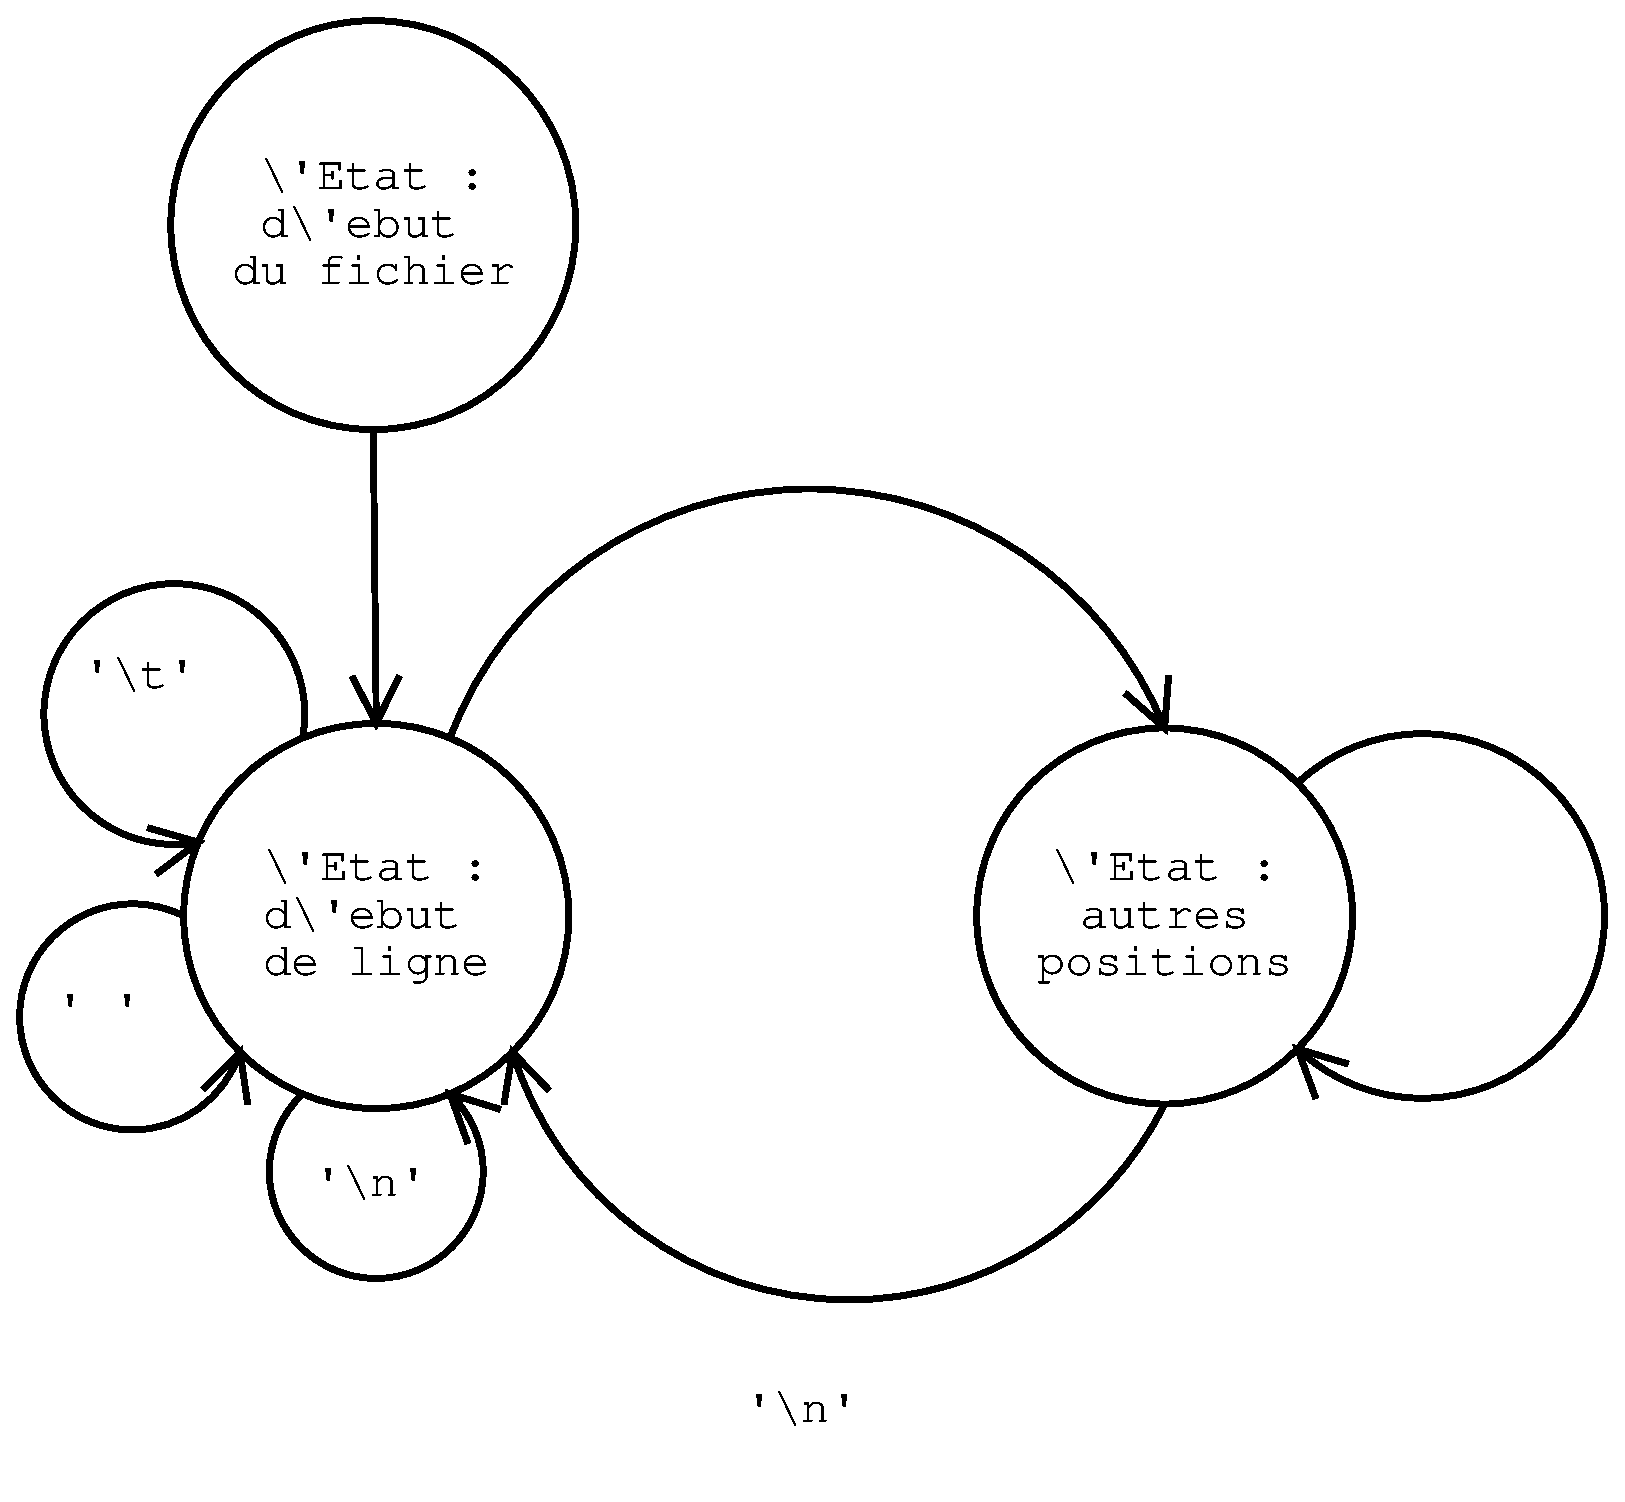
\includegraphics[scale=.3]{../Illustration/automatepp}  
%END LATEX
%HEVEA  \epsfbox{automatepp.ps}  
\end{center}
\begin{exercice}[Construction d'un programme \`a partir d'un automate]
  Inspirez vous de cet automate pour \'ecrire un filtre qui supprime
  les espaces ou les tabulations en d\'ebut de chaque ligne.
   \ifcorrection%
   \begin{correction}
\begin{verbatim}
     #include <stdio.h>
#include <stdlib.h>

int 
main()
{
    int c;
    enum {ETAT_DBT_LIGNE, ETAT_NORMAL } etat = ETAT_DBT_LIGNE;
  
    while ((c=getchar()) != EOF) {
        switch (etat) {
            case ETAT_DBT_LIGNE:
                switch (c) {
                    case ' ':
                    case '\t':
                        break;
                    default:   
                        putchar(c);
                        etat = ETAT_NORMAL;
                        break;
                }
                break;
            case ETAT_NORMAL:
                switch (c) {
                    case '\n': 
                        putchar('\n');
                        etat=ETAT_DBT_LIGNE;
                        break;
                    default :  
                        putchar(c);
                        break;
                }
        }
    }

    exit(EXIT_SUCCESS);
}
\end{verbatim}
   \end{correction}
   \fi%
\end{exercice}

\subsection{Le travail restant \`a faire}
Construisez l'automate codant nos r\`egles de styles et implantez le.

